\documentclass[times, 10pt]{thesisMDH}
\usepackage[ddmmyyyy]{datetime}
\usepackage[pdfborder={0 0 0},colorlinks=true,urlcolor=blue,citecolor=red,bookmarks=false]{hyperref}
\usepackage{float}
\usepackage{makecell}
% \usepackage{indentfirst}
\setlength\parindent{0pt}

\university{University of Science and Technology of Hanoi}
\department{Information and Communication Technology}

\subject{Distributed System}
\thesisTitle{Practical Work 6:\\GlusterFS}

\authorOne{Nguyen Phuong Thao}{BI9-212}
\authorTwo{Doan Tuyet Mai}{BI9-162}
\authorThree{Trinh Thao Phuong}{BI9-191}
\authorFour{Phung Kim Son}{BI9-202}
\authorFive{Pham Minh Long}{BI9-146}

\theDate{Hanoi, Mar 2021} 

\begin{document}
\titlePage

\newpage

\mainmatter

\section{System organization}
\begin{figure}[H]
    \centering
    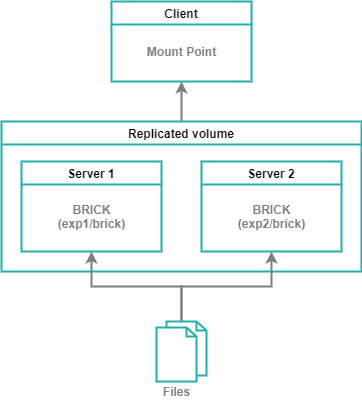
\includegraphics[width = 0.6\linewidth]{images/img61.png}
    \caption{System organization}
\end{figure}
Gluster is a scalable, distributed file system that aggregates disk storage resources from multiple servers into a single global namespace. In this implementation, we created three virtual machine, two of them are servers which play the role of bricks in the replicated volume and a virtual machine is the client which is a mount point of the replicated volume. By default TCP protocol will be used by GlusterFS to transfer the files between the client and the volume.

\section{Implementatation}
In this labwork, we used the 3 virtual machines to act as the servers and client to perform the distributed replicated volume using GlusterFS. Each machine was set to 1 CPU, 1 GB of RAM and using Ubuntu 20.04 LTS, they connected each other via internal network.
\subsection{Configuring the Host File}
The first step we need to do before installing glusterfs on all servers is configuring the hosts’ file.
\begin{lstlisting}
sudo nano /etc/hosts
\end{lstlisting}
And then we add the IP of all servers, client to the host file of each machine. In this case, 2 servers (server,client) have the IP address 192.168.115.1 and 192.168.115.2, respectively. The client has the IP address 192.168.115.3
\begin{lstlisting}
192.168.115.1   server
192.168.115.2	client
192.168.115.3	client-new
\end{lstlisting}

\subsection{Installing GlusterFS Server, Configuring GlusterFS Servers}
The second step is to install and configuring the GlusterFS in each server.\\
To install GlusterFS, we follow the steps:
\begin{lstlisting}
sudo apt install software-properties-common
sudo add-apt-repository ppa:gluster/glusterfs-7
sudo apt update
sudo apt install glusterfs-server
\end{lstlisting}
Next, in the both server, we need to enable the \texttt{glusterd} service as the following command
\begin{lstlisting}
sudo systemctl start glusterd
sudo systemctl enable glusterd
\end{lstlisting}
From the server 1 (server), the server 2 (client) could be added to the storage trusted pool by the command
\begin{lstlisting}
sudo gluster peer probe client
\end{lstlisting}
To check the storage pool status
\begin{lstlisting}
sudo gluster pool list
\end{lstlisting}
And here is the output result
\begin{figure}[H]
    \centering
    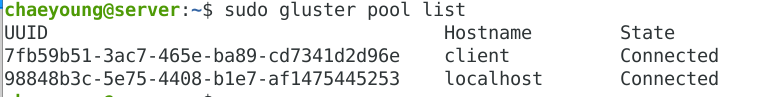
\includegraphics[width=0.7\linewidth]{images/cap1.png}
\end{figure}

\subsection{Setting up the Distributed GlusterFS Volume}
First, we created new directory \texttt{/glusterfs/test} on both 2 servers
\begin{lstlisting}
sudo mkdir -p /glusterfs/test
\end{lstlisting}
Then in the server 1 (server), we created the distributed glusterfs volume named \texttt{voltest} with 2 replicas \texttt{server} and \texttt{client}
\begin{lstlisting}
sudo gluster volume create voltest transport tcp server:/glusterfs/test client:/glusterfs/test force
\end{lstlisting}
Before accessing the data, we need to first start the volume
\begin{lstlisting}
sudo gluster volume start voltest
\end{lstlisting}
And here is the information of the volume \texttt{voltest} after creation
\begin{figure}[H]
    \centering
    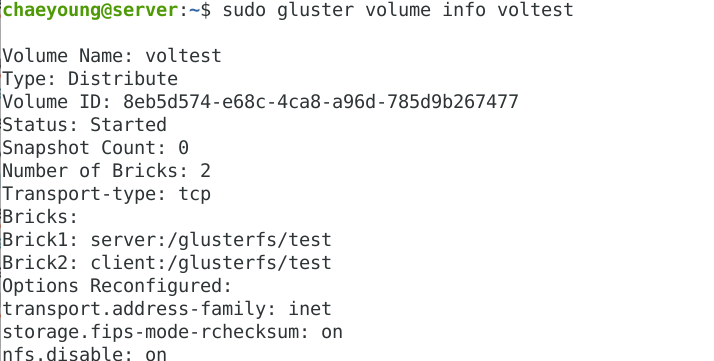
\includegraphics[width=0.7\linewidth]{images/cap2.png}
\end{figure}

\subsection{Configuring GlusterFS Client}
First, we need to install \texttt{glusterfs-client} package.\\
Then, we created a new directory \texttt{/mnt/glusterfs} and then, mounted the distributed glusterfs volume \texttt{voltest} to the \texttt{/mnt/glusterfs} directory. 
\begin{lstlisting}
sudo mkdir -p /mnt/glusterfs
sudo mount -t glusterfs server:/voltest /mnt/glusterfs
\end{lstlisting}
And here is result
\begin{figure}[H]
    \centering
    
\includegraphics[width=0.7\linewidth]{images/cap3.png}
\end{figure}

\section{Benchmark}
First, we created 2 test file, one is \texttt{file1.txt} with a small size of 6 bytes and \texttt{file3.txt} with a size of 524 KB.
\begin{lstlisting}
sudo touch file1.txt file2.txt
\end{lstlisting}
And the following figures are the implementation of measuring the file I/O
\begin{figure}[H]
    \centering
    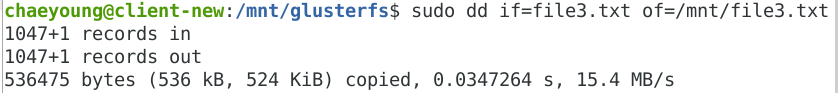
\includegraphics[width=0.7\linewidth]{images/cap4.png}
\end{figure}
\begin{figure}[H]
    \centering
    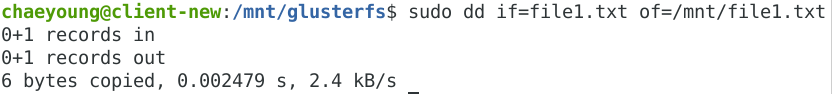
\includegraphics[width=0.7\linewidth]{images/cap5.png}
\end{figure}
As we can see here, the first text file has a very small size, as a result, the read speed is slow.


\section{Contribution}
\begin{center}
    \begin{tabular}{|l|l|l|}
        \hline
        \textbf{Student} & \textbf{Student ID} & \textbf{Contribution}\\
        \hline
        Pham Minh Long & BI9-146 & Write report\\
        \hline
        Phung Kim Son & BI9-202 & GlusterFS implementation\\
        \hline
        Trinh Thao Phuong & BI9-191 & Write report \\
        \hline
        Doan Tuyet Mai & BI9-162 & Implement benchmark \\
        \hline
        Nguyen Phuong Thao & BI9-212 & Research for GlusterFS\\
        \hline
    \end{tabular}
\end{center}

\end{document}